\chapter{提案モデルによる日本近辺の風速予測\label{chap:experiments}}
本論文では,提案モデルの性能検証のために日本近辺の風速予測を実施した.また,性能の比較のためにCNNによるエンコーダ・デコーダとLSTMを用いたU-Net-likeなモデルを実装し,それぞれのモデルの性能を比較した.

\section{実験の概要 \label{section:exp-overview}}
ここに何をメトリクスとして取ったのかとかを書く

\section{利用したデータ及び学習条件 \label{section:exp-data-and-condition}}
\subsection{利用したデータ \label{subsection:exp-data}}
気象庁が提供している日本近辺の風速と気圧データを京都大学の生存圏データベース\cite{Seizonken2004}から入手した.このデータセットは図\ref{fig:exp-data-overview}に示す通り,日本近辺の北緯$22.4\tcdegree$から$47.6\tcdegree$まで,東経$120\tcdegree$から$150\tcdegree$までの領域をそれぞれ$0.05\tcdegree \times 0.0625\tcdegree$の細かさで等緯度等経度に区切り,各格子点上における風速と気圧を記録したものである\cite{JMBSC2022}.すなわち,ある一時刻のデータは緯度経度について$505 \times 480$の行列となっており,ある一点には風速の南北方向成分$(\mathrm{m/s})$, 風速の東西方向成分$(\mathrm{m/s})$, 気圧$(\mathrm{hPa})$の3つの値が記録されている.
\begin{figure}[bp]
  \centering
  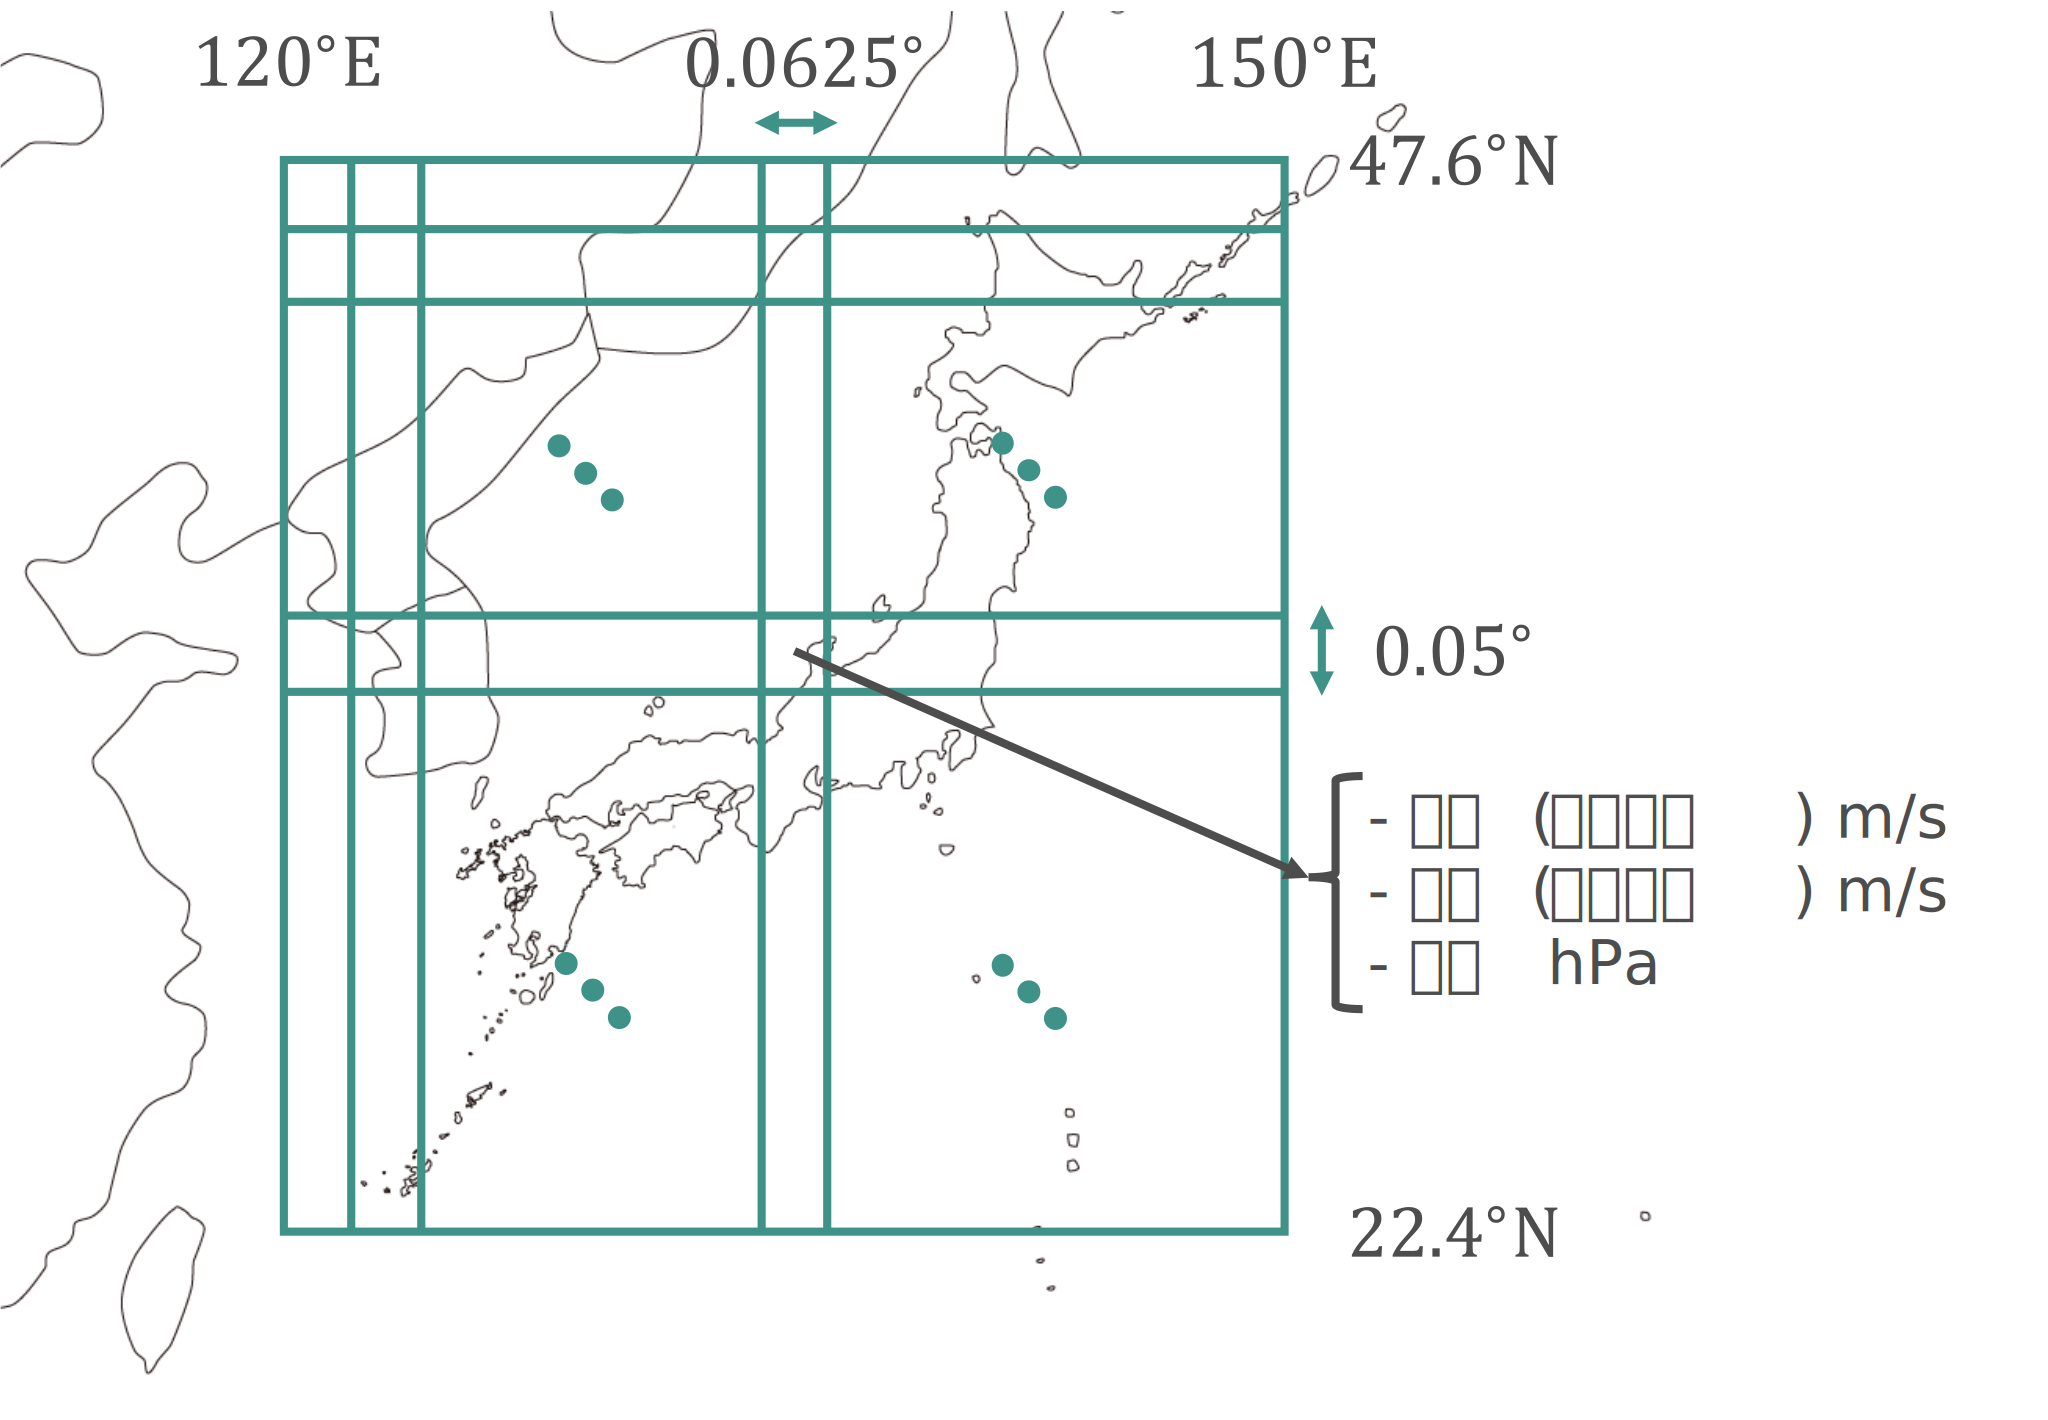
\includegraphics[width=0.6\linewidth]{./experiments/figs/data_overview.svg.eps}
  \caption{気象庁が提供している日本近辺の風速と気圧データの領域}
  \label{fig:exp-data-overview}
\end{figure}

今回の時系列データは3時間間隔であり,(前日の)21:00, 0:00, 3:00の3時刻分のデータを入力として6:00の時刻の風速を予測するというタスクを行った.すなわち,式(\ref{eq:time-series-input})において$n=5$,式(\ref{eq:time-series-t})において無次元時刻$\Delta T$は$3[\mathrm{h}]$相当である.この4時刻分の時系列データを2011年1月1日から2020年12月31日までの3650日分用意し(統計を取る際の簡便化のために閏日は除いてある),\ref{subsection:exp-data-preprocessing}で述べる処理をする前の全体のデータセットとした.

処理前の全体のデータセットの詳細な統計量を表\ref{todo:table:exp-pre-data-statistics}に示す.

\subsection{データの前処理 \label{subsection:exp-data-preprocessing}}
\ref{subsection:exp-data}項で述べたデータセットをそのまま入出力として用いるのではなく,いくつかの前処理を実施した.その処理の詳細を以下に示す.

まず図\ref{fig:exp-averaging}に示すように,$505 \times 480$の行列を更に$10 \times 10$の格子によって区切り,この格子内で風速と気圧を平均化することで$50 \times 48$のサイズまで落とした.なお,端数分は切り捨てている.これは,提案モデルの格子の大きさを適切に設定することで,3時間で変化する風速の空間的な変化を捉えることができると考えたためである.このデータセットを改めて全体のデータセットとした.このデータセットの詳細な統計量を表\ref{todo:table:exp-data-statistics}に示す.

\begin{figure}[bp]
  \centering
  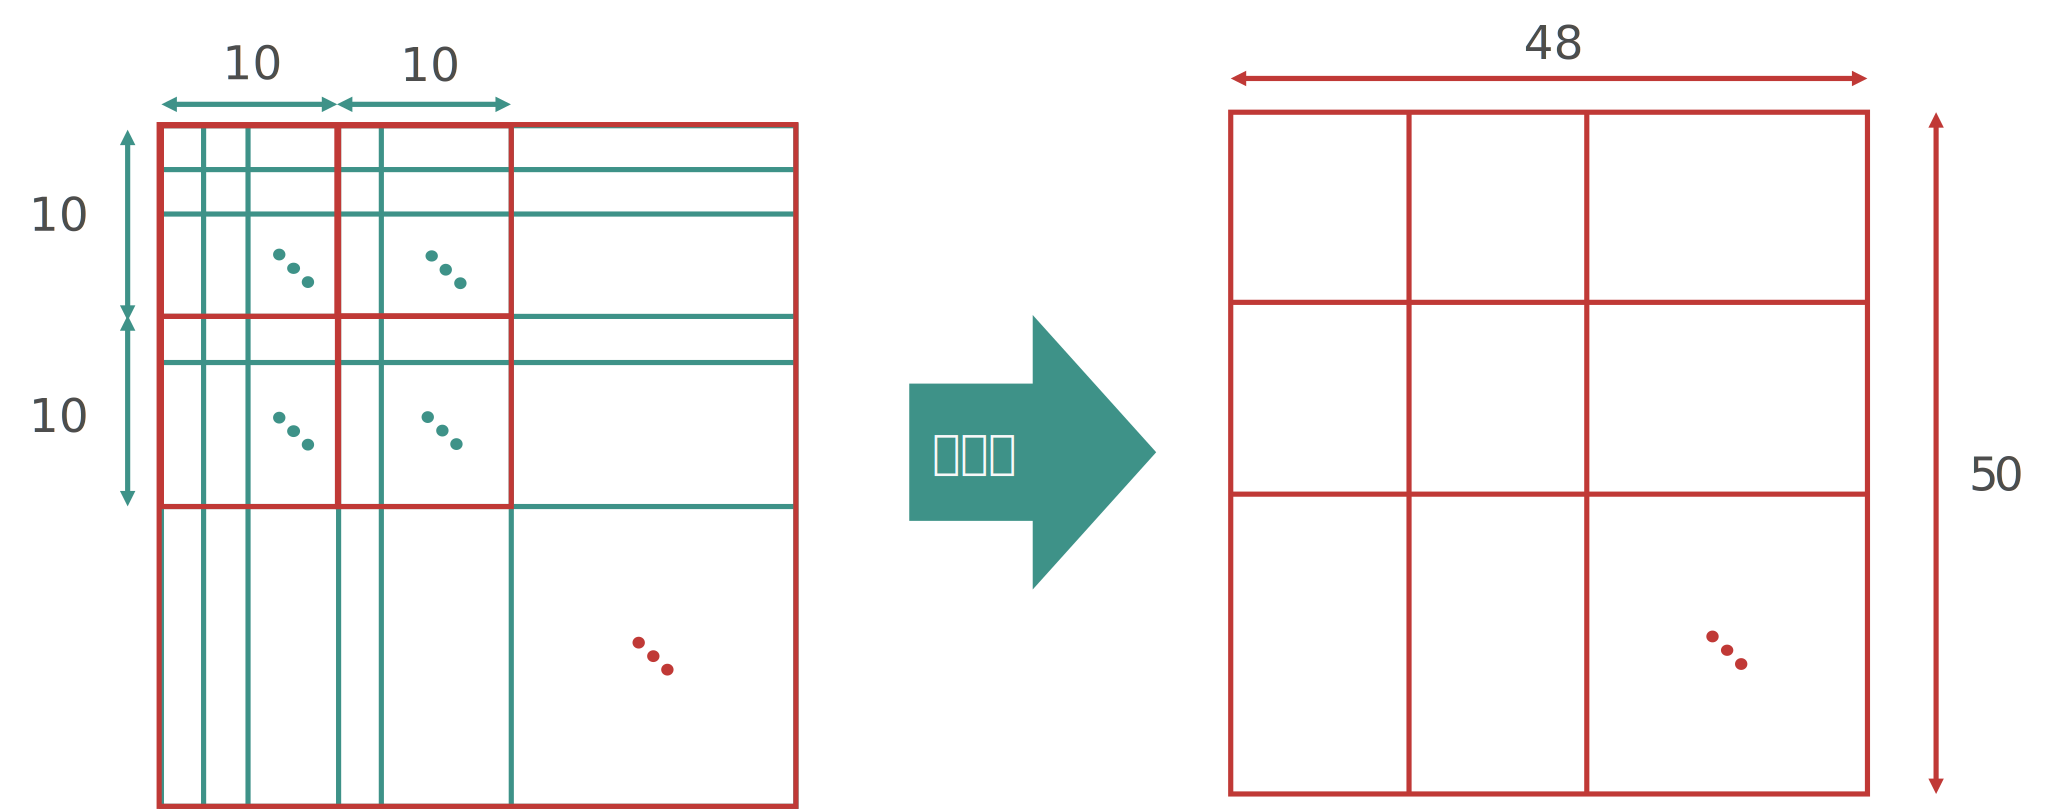
\includegraphics[width=0.8\linewidth]{./experiments/figs/average_pool.svg.eps}
  \caption{風速と気圧の平均化}
  \label{fig:exp-averaging}
\end{figure}

%todo 標準化についても時間があればここで触れる

\subsection{学習条件 \label{subsection:exp-condition}}

続いて,モデルの詳細な学習条件について述べる.まず,提案モデルの原理について\ref{subsection:time-series-model}項で述べたがここでは具体的な数値を示しながらモデルのアーキテクチャを見る.図\ref{fig:exp-model-architecture}に示したように,このモデルでは並進と衝突をそれぞれ5回行った(緑の実線矢印が並進を表し,緑の破線矢印が衝突を表している).すなわち式(\ref{eq:time-series-t})において$\Delta T = 5$である.\ref{subsection:time-series-less-model}項で述べた通り衝突の回数分だけ外枠が削られるため,図中の赤破線によって強調しているように出力層の大きさは入力層に比べて東西南北の端$5$マス分減少している.

\begin{figure}[bp]
  \centering
  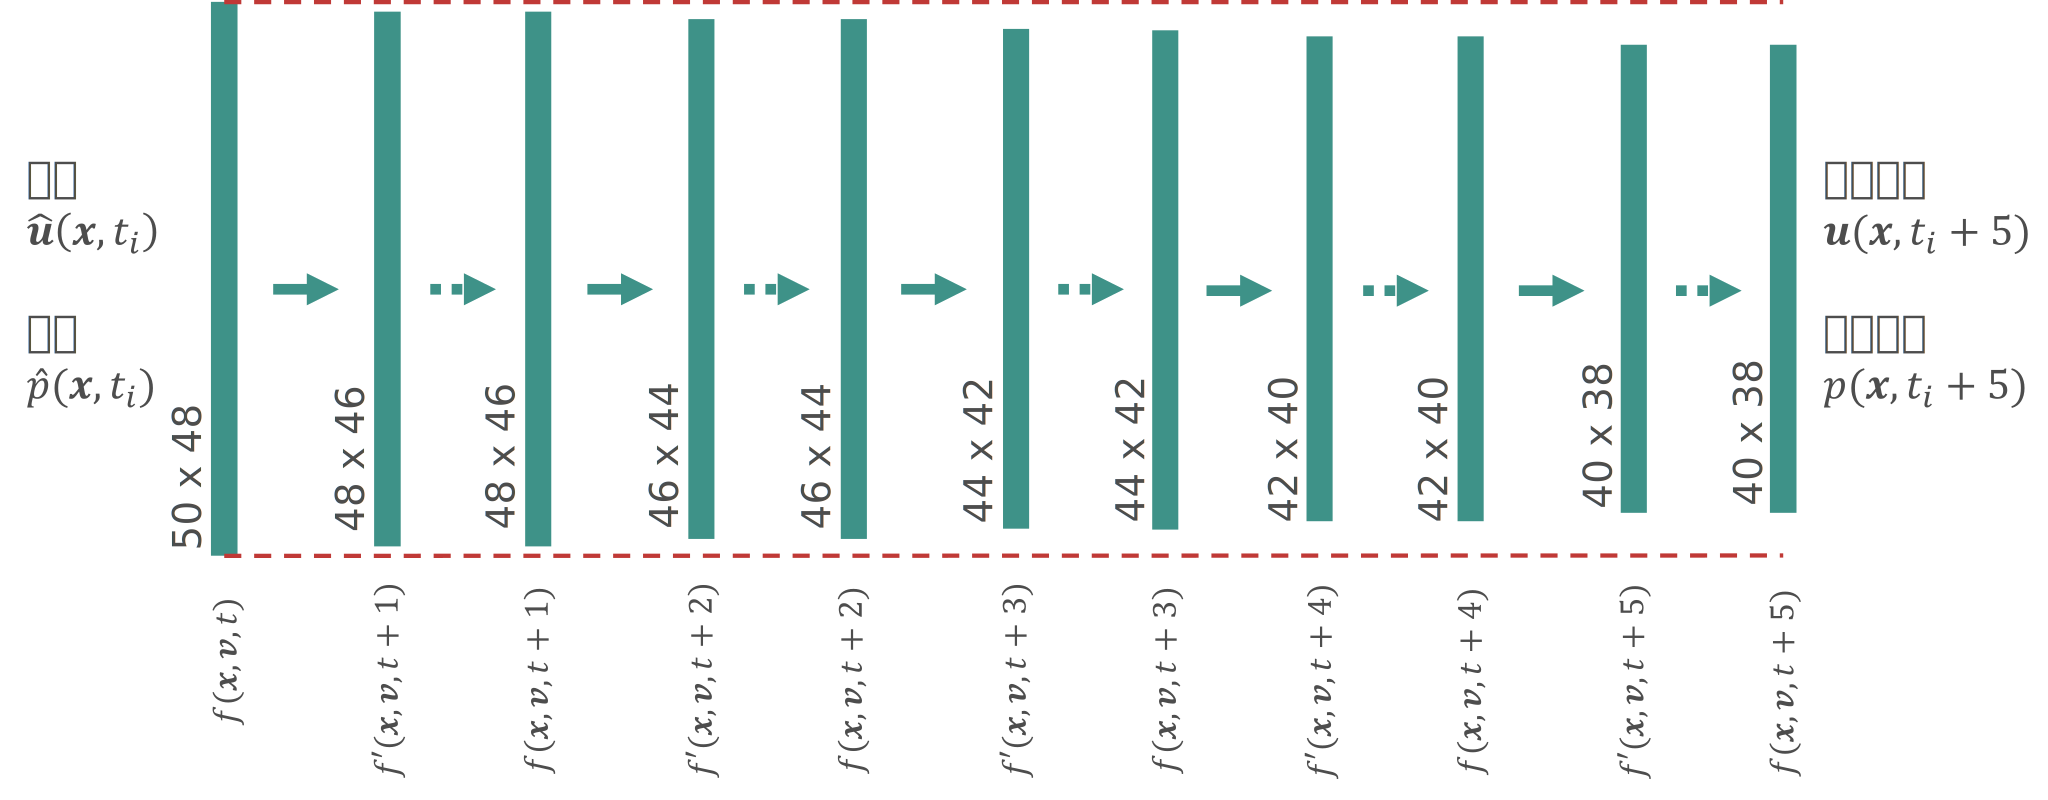
\includegraphics[width=0.85\linewidth]{./experiments/figs/model_architecture.svg.eps}
  \caption{モデルのアーキテクチャ}
  \label{fig:exp-model-architecture}
\end{figure}

% 損失関数について,式(\ref{eq:time-series-loss})に示したがここでは風速の精度を重視するため,式(\ref{eq:time-series-loss})の第1項の重みを$1$,第2項の重みを$0.1$とした.
%todo: なんで気圧の予測はしないのか聞かれたらこの辺も追記する

提案モデルの学習にはAdam\cite{Kingma2014AdamAM}を用いた.学習率は$10^{-3}$とし,ミニバッチサイズは$16$とした.全体のデータセットを2920日分と730日分に分けそれぞれを学習用データと検証用データとした.学習は$500$エポック行い,かかった時間は約8時間であった.実行環境にはGoogle Colaboratory\cite{GoogleColaboratory}を用い,GPUはTesla T4を用いた.また提案モデルの構築にはPyTorch\cite{NEURIPS2019-9015}を用い,自動微分による学習を行った.
% 損失の重み付けについて書く(速度に重みを強くつけた)

% 学習するLBM
% 学習しないLBM
% U-Net-Like
% で,
% 全体のRMSE, ME
% 座標ごとのRMSE, ME 東西方向, 南北方向,風速, 風向
% 時間ごとのRMSE, ME 上のそれぞれ
% 特徴的な日の座標のRMSE, ME 上のそれぞれ
% 
% それぞれのRMSE比についても書く(4.4のほうかな?)

\section{実験結果 \label{section:exp-results}}

\section{物理的な構造を含まない深層学習モデルによる実験結果 \label{section:exp-results-without-physicial-structure}}

\section{考察 \label{section:exp-discussion}}
% 平均化についてもふれて,どうやってアップスケーリングするか
% 短所として外枠の風速が予測できないことにふれる